\chapter{Diseño y arquitectura del sistema}\label{diseno}

En este capítulo se abordará el diseño del sistema. Para ello, a partir del estudio de los métodos y procedimientos disponibles en 
Bro para la gestión de flujos, se determinarán los módulos y funcionalidades necesarias, proponiéndose una arquitectura para el 
sistema a implementar.

\intro Así, en primer lugar se presentará la arquitectura propuesta y los diferentes módulos y funcionalidades. También se describirán 
las estructuras de datos usadas para la gestión de la información.

\section{Arquitectura del sistema}

Para describir la arquitectura del sistema hay que tener en cuenta la arquitectura de Bro. Este monitor de red es un software modular, 
esto es, esta compuesto de diferentes módulos que al ser ejecutados funcionan como un único sistema.

\intro Por lo tanto, la arquitectura del sistema a desarrollar se debe de acoplar a la arquitectura propia de Bro, por lo que el 
sistema debe implementarse como un módulo adicional compatible. Entre los requisitos del mismo se encuentra que sea ligero y 
eficiente. Por lo tanto, se deberán usar los distintos eventos y capacidades que proporciona Bro para minimizar el impacto en el 
sistema global y optimizar su funcionamiento.

\intro Se prescindirá del uso de los \textit{frameworks} descritos en el capítulo anterior (\ref{sub.framew}), pues su uso no aporta 
nada relevante que no se pueda realizar exclusivamente con los eventos ya disponibles destinados a gestionar el tráfico de la capa de 
transporte. Así, se propone usar este tipo de eventos como núcleo y soporte del módulo y de todas las funcionalidades necesarias. Las 
dos funcionalidades más relevantes del módulo están relacionadas con la evaluación de la similitud entre flujos y la gestión de las 
listas de flujos en diferentes situaciones. Así, se definirá una función que se encargará de evaluar la fórmula del emparejamiento de 
flujos (Apartado \ref{sec.emparejamiento}). Esta función devolverá un número que será el que se compare con el umbral.

\intro En la Figura \ref{fig.digsistema}, se pueden ver los distintos pasos que se seguirán en la ejecución del módulo, siendo estos 
complementados por los pasos que se ven en las Figuras \ref{fig.calculo} y \ref{fig.emparejamiento}, de la siguiente sección.

\begin{figure}[H]
  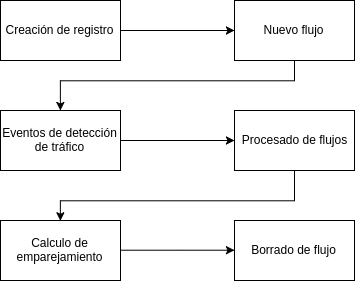
\includegraphics[width=0.75\textwidth]{imagenes/DiagramaSistema.png}
  \centering
  \caption{Diagrama del sistema.}\label{fig.digsistema}
\end{figure}

\intro De esta forma, se creará un registro en el cual se almacenarán los flujos que son emparejados. De esta forma se evita tener 
que iterar sobre la tabla de emparejados al finalizar el módulo, haciendo que la ejecución sea más eficiente.

\intro En la Figura \ref{fig.nacimiento}, se puede ver cómo se procederá a analizar un flujo cuando es detectado. En primer lugar se 
detectará el flujo y se iniciará la búsqueda de otro con sus características, en caso de que se encuentre, se comenzará con el 
análisis. Si no se detecta ningún flujo con sus parámetros, se almacenará.

\begin{figure}[H]
  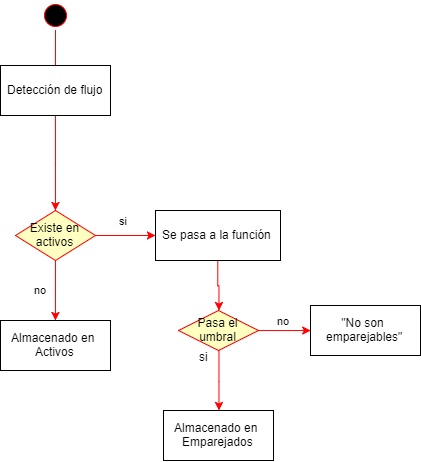
\includegraphics[width=0.5\textwidth]{imagenes/nacimiento.png}
  \centering
  \caption{Detección de un nuevo flujo.}\label{fig.nacimiento}
\end{figure}

\intro En la Figura \ref{fig.muerte}, se puede ver cómo se comportará el sistema cuando vaya a eliminar un flujo de la memoria. Se 
buscará un flujo en la lista de activos para que lo reemplace, en caso de que no haya ninguno con sus características se borrará de la 
memoria.

\begin{figure}[H]
  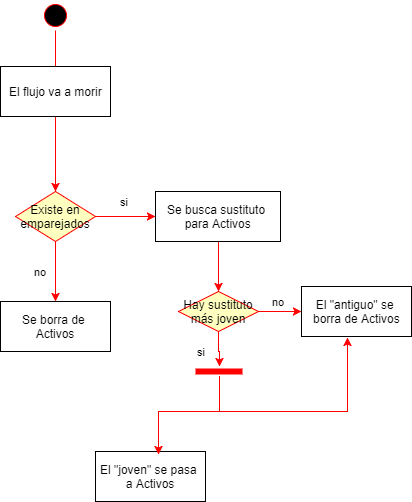
\includegraphics[width=0.5\textwidth]{imagenes/muerte.png}
  \centering
  \caption{Muerte de un flujo.}\label{fig.muerte}
\end{figure}

\intro Dependiendo del trato que se les vaya a dar a los flujos detectados, se almacenarán en una lista o en otra. Estos pueden estar 
en diferentes estados, siendo estos los que se consideran:

\begin{itemize}
\item Activo. El flujo está activo y almacenado.
\item Emparejado. El flujo ha sido emparejado con otro flujo activo.
\item Finalizado. El flujo ha cumplido su tiempo de vida y es borrado de la memoria.
\end{itemize}

\intro Por lo tanto, cuando un flujo es detectado tendrá el estado activo. En función 
de los distintos flujos que se vayan detectando, los que están en estado \textit{activo} se irán comparando con los nuevos que se detecten, de modo que los nuevos pasarán a estar emparejados. Si no se encuentra un flujo activo que coincida con sus parámetros, los nuevos flujos serán almacenados como activos. Al último estado, finalizado, se podrá pasar tanto del estado activo, como del emparejado, con la diferencia de que, de tratarse del primer caso, deberá de ser borrado de la lista y se buscará un sustituto entre los emparejados con ese flujo. En el segundo caso no se borrará de la lista. La transición de estados se puede ver en la Figura \ref{fig.flujos}.

\begin{figure}[H]
  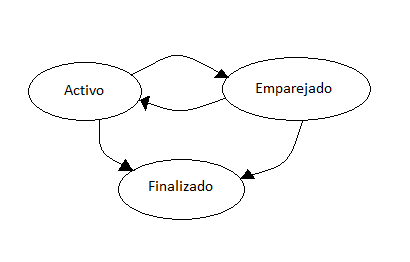
\includegraphics[width=0.7\textwidth]{imagenes/flujos.png}
  \centering
  \caption{Distintos estados de los flujos.}\label{fig.flujos}
\end{figure}

\intro Para el análisis, será necesario disponer de tráfico. Este entrará en forma de traza con formato \textit{pcap}. Las salidas 
se darán en forma de registros, en los cuales se mostrarán los flujos que han sido emparejados.

\intro La configuración de Bro, se realiza mediante la línea de comandos, cuando se va a lanzar el programa. Por lo tanto, para el 
módulo que se está describiendo es preciso únicamente activar la opción \textit{-r}, de forma que se le permita leer el archivo que se 
le pasará como parámetro a continuación. En el caso de que se quiera escanear el tráfico de una interfaz, se deberá de activar la 
opción \textit{-i} indicando a continuación el nombre de la interfaz a analizar. Se puede ampliar esta información leyendo la ayuda de 
Bro con \textit{-h} o en el apéndice \ref{cap.uso}.

\section{Módulo y funciones}

Las funcionalidades que se espera que tenga este módulo en esencia son dos, la detección y almacenado 
del tráfico, y la aplicación de la fórmula para conocer si dos flujos son emparejables. Aunque estas son las dos funcionalidades 
básicas, también será necesario disponer de algunas funcionalidades extra. De una forma más amplia las funciones del módulo serán las 
siguientes. 

\begin{itemize}
\item \textit{Función que aplique la fórmula de emparejamiento}. 
\intro A esta función se le pasará dos flujos, de forma que se aplique la fórmula y devuelva un número, el cual 
será el que indique si los flujos son emparejables o no.
\item \textit{Función de preprocesado}. 
\intro Esta función se encargará de indicar si dos flujos son candidatos a ser emparejados o no. Si son candidatos, se llamará a la función de emparejamiento, de forma que con el resultado que devuelva se decida si se almacenan como emparejables o no.
\intro En el uso de esta función se almacenará o no el flujo que está siendo analizado. Por lo tanto será necesario el uso de algún tipo de contenedor para este cometido.
\item \textit{Funciones que detecten el tráfico}. 
\intro Esto se hará con los eventos de Bro. Los eventos detectarán el tipo de tráfico que se está analizando y llamarán a la función 
anterior.
\item \textit{Creación de registro}.
\intro A su vez, será necesario crear un registro o \textit{log} con la información que aporta el sistema de identificación.
\end{itemize}

\intro En la Figura \ref{fig.calculo}, se puede ver cómo se realizará el preprocesado de un flujo antes de aplicar la ecuación de emparejamiento \ref{ecug}.

\begin{figure}[H]
  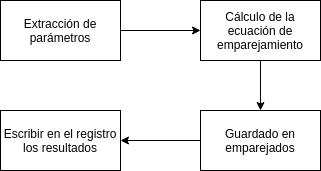
\includegraphics[width=0.6\textwidth]{imagenes/calculo.png}
  \centering
  \caption{Diagrama de la función previa a la aplicación de la ecuación de emparejamiento.}\label{fig.calculo}
\end{figure}

\intro En la Figura \ref{fig.emparejamiento}, se ve cómo se tratan a los flujos que han pasado el preprocesado y que son candidatos a ser emparejados.

\begin{figure}[H]
  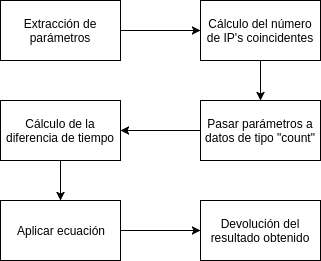
\includegraphics[width=0.6\textwidth]{imagenes/emparejamiento.png}
  \centering
  \caption{Diagrama de aplicación de la función de emparejamiento.}\label{fig.emparejamiento}
\end{figure}


\intro Lo que se espera es capturar el tráfico de la capa de transporte. Dicho tráfico se corresponde a los 
protocolos \textit{TCP y UDP}. Por lo tanto será necesario ver que tipo de eventos son los que controlan el tráfico 
de estos dos protocolos. A su vez, se tendrá que crear variables globales para el almacenamiento de los flujos que sean emparejables 
y los que estén activos.

\intro Las entradas y salidas son de fácil gestión. Las entradas de tráfico podrán ser mediante archivos o 
analizando directamente el tráfico de la red. Las salidas, por su parte, se realizarán mediante registros. Con esto, se guardará en un fichero en la ruta donde es lanzado el monitor, siendo el posterior análisis mucho más cómodo desde, por ejemplo, un editor de texto.

\intro Se debe de tener en cuenta que siempre se podrá extender la funcionalidad del módulo. Pero de momento no 
resulta interesante. La posible extensión correspondería a posibles trabajos futuros.

\intro Para realizar este módulo es necesario conocer como gestiona los flujos Bro y de que forma se mantendrán 
los que son emparejados y los que están activos.

\section{Gestión de flujos}

La gestión de los flujos se realiza completamente mediante los eventos de Bro.

\intro Existen eventos que gestionan el nacimiento y la muerte de los flujos, siendo estos dos eventos genéricos. Por el contrario, 
se deberán de usar los distintos eventos especializados para gestionar los distintos tipos de tráfico.

\intro De esta forma, se tendrán eventos únicos que detectarán el tráfico \textit{TCP} y otros para \textit{UDP}. Una vez dentro, se 
realizarán los pasos necesarios para llevar el flujo detectado hasta la función de evaluación.

\intro En el evento correspondiente al nacimiento de un flujo, se deberá de analizar si se tiene otro con el que compararlo, o directamente se almacena con los demás flujos activos.

\intro En cuanto al evento relacionado con la muerte de un flujo, se tendrá que evaluar si en la lista de emparejados se tiene otro, al cual le quede más tiempo de vida, para que lo reemplace en la lista de flujos activos.

\intro A continuación se verán las estructuras de datos necesarias para llevar a cabo el desarrollo del módulo.

\section{Estructuras de datos}

Las principales estructuras de datos que se necesitan para el desarrollo de este trabajo serán dos tablas, \textit{table} 
\cite{brotable}, de vectores para el almacenamiento de los flujos activos y los emparejados. Los vectores son iguales que en cualquier 
otro lenguaje de programación, mientras que las tablas son parecidas a los \textit{maps} de \textit{C++}. Aunque esto se explicará más 
detalladamente en el capítulo \ref{implementacion}.

\intro Dichas estructuras de almacenamiento, deberán de ser capaces de estar ordenadas por las IP's y los puertos. Esto se obtiene 
haciendo que las tablas estén compuestas de vectores, por lo cual, se obtendrá una matriz bidimensional indexada. Por lo tanto se 
consigue que el acceso a los datos sea mucho más rápido. Incluso se podría prescindir de bucles, los cuales pueden acabar 
siendo un problema en cuanto a rendimiento si se analiza mucho tráfico. En la Figura \ref{fig.tablas}, se muestra cómo están 
organizadas las matrices.

\begin{figure}[H]
  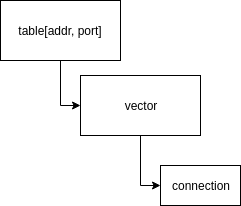
\includegraphics[width=0.4\textwidth]{imagenes/tablas.png}
  \centering
  \caption{Organización de las tablas.}\label{fig.tablas}
\end{figure}

\intro Bro proporciona cierto tipos de datos muy interesantes, los cuales además, incluyen mucha más información. Algunos de estos 
tipos de datos son. 

\begin{itemize}

\item \textit{connection}. 

\intro Este tipo de dato es el flujo en sí. Por lo tanto será de vital importancia comprenderlo para poder trabajar como se desea.

\intro Dentro de \textit{connection} existe un registro llamado \textit{id}, el cual esta compuesto por el tipo de dato \textit{conn\_id} \cite{broconnid}. Este dato sirve para identificar los flujos mediante una tupla formada por 4 datos. Estos datos son los que se 
precisan para indexar la matriz bidimensional. En la Figura \ref{fig.connection} se muestran los dos datos que se usarán de \textit{connection}.

  \begin{itemize}

  \item \textit{addr}. Este tipo de dato representa una IP. Reconoce tanto IPv4 como IPv6. Este tipo de dato puede 
  ser comparado e incluso ordenado mediante operadores \cite{broaddr}.

  \item \textit{port}. Este tipo es el usado para los puertos. Además del número, también indica el 
  protocolo de la capa de transporte que usa. Soporta la comparación y ordenación, pero no por el número, sino por 
  el tipo de protocolo \cite{broport}.
  \end{itemize}

\begin{figure}[H]
  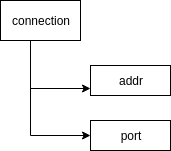
\includegraphics[width=0.4\textwidth]{imagenes/connection.png}
  \centering
  \caption{Tipo connection desglosado.}\label{fig.connection}
\end{figure}

  
\intro Se puede consultar más información sobre el tipo de dato \textit{connection} en \cite{connectiontype}.

\item \textit{time}. 

\intro Aunque en otros lenguajes se pueden crear estructuras que se asemejen a este tipo, Bro da un tipo de dato muy completo. Además, 
se puede operar sobre él desde el principio, siendo una gran ventaja a la hora de calcular el tiempo de inicio de los flujos. Más 
información en \cite{timetype}.

\intro Es importante entender que para realizar el cálculo para el emparejamiento de flujos, se necesita el 
\textit{timestamp} del primer paquete de cada flujo, pues será sobre este tiempo sobre el que se apoye el 
cálculo del emparejamiento.

\end{itemize}

\intro Estos dos tipos de datos a parte de ser los más interesantes para el cálculo del emparejamiento, también 
serán los más utilizados junto a los contenedores para los flujos. Existen más tipos de datos e incluso los hay que 
extienden la información disponible sobre los flujos. Más información sobre distintos tipos de datos en \cite{conntype}.
